\scanpage{57}
% archive sheet number: 56

% L1–4, upper left
\figure{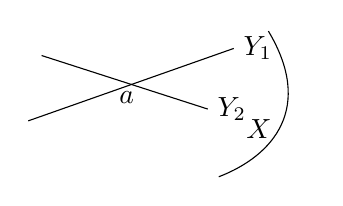
\begin{tikzpicture}[x=1cm,y=1cm]\draw (-1.25,-.47)--(1.36,.45) node[right] {$Y_1$};\draw (-1.08,.36)--(1.03,-.32) node[right] {$Y_2$};\node[below] at (0,.02) {$a$};\draw (1.80,.67) .. controls (2.38,-.30) and (1.87,-.91) .. (1.17,-1.18);\node at (1.68,-.58) {$X$};\end{tikzpicture}}

% L1–12, extending the section
Soit $F$ le faisceau \inserted{sur \deleted{\unsure{$X$}}} des applications \unsure{quelc.} dans $\mathbb{Q}$, et $Y'=Y-\{a\}$, considérons la section de $F|Y'$ qui est $0$ sur $Y'_1$, $1$ sur $Y'_2$, on ne peut la prolonger à $Y$, car \unsure{si on|si l'on} pouvait, il y aurait un voisinage ouvert $U$ de $a$, et une application $U\longrightarrow\mathbb{Q}$ qui \deleted{\unsure{en les pts de} $Y'_1$ ($Y'_2$) \unsure{serait}} au voisinage de $Y'_1$ ($Y'_2$) induirait $0$ ($1$), absurde car ces voisinages doivent se couper !

% L13–17, cancelled development
\deleted{On ne peut cependant s'en tirer avec $Y$ une \uline{courbe} pour \unsure{contre-exempler} le pb du début. En \unsure{effet}, décomposant $Y$ en ses composantes \inserted{irr.} $Y_i$, on aurait un}

% L17, cancelled sequence
\[
\deleted{F_{\deleted{\unsure{Y}}Y}\longrightarrow\prod_i F_{Y_i}\longrightarrow G\longrightarrow0},
\]

% L18–19, cancelled continuation
\deleted{$G$ concentré en un ens fini, d'où \deleted{$H^{\unsure{1|0}}$} (les $F_{Y_i}$ étant flasques, d'où $H^1(Y,F_{Y_i})=0$]}

% L20, cancelled cohomology sequence
\[
\deleted{\deleted{\unsure{H^1(}}\quad\prod_i H^0(\unsure{X|Y|Y_2},F_{Y_i})\longrightarrow \deleted{\unsure{G}}H^0(Y,G)\longrightarrow H^1(Y,F_Y)\longrightarrow 0}
\]
